\documentclass[11pt]{article}
\usepackage[a4paper, margin=2.54cm]{geometry}
\usepackage[utf8]{inputenc}
\usepackage{babel}
\usepackage[spanish]{layout}
\usepackage[article]{ragged2e}
\usepackage{textcomp}
\usepackage{amsmath}
\usepackage{amssymb}
\usepackage{amsfonts}
\usepackage{proof}
\usepackage{enumerate}
\usepackage{graphicx}
\usepackage{multirow}

\setlength{\parindent}{0pt}

\title{
    Entrega 2 \\
    \large Sistemas Operativos II}
\author{Mellino, Natalia \and Farizano, Juan Ignacio}
\date{}

\begin{document}
\maketitle

\noindent\rule{\textwidth}{1pt}

\section*{Ejercicio 1}

Los procesos alternan entre ráfagas (o \emph{bursts}) en las que realizan cómputo interno
y otras, en donde están limitados por operaciones de entrada/salida (\emph{I/O bound}). 
En estos últimos la atención del planificador desaparece ya que el proceso deja de
estar \textbf{listo} y pasa a estar \textbf{bloqueado}. Entonces, si bien los procesos están en ejecución un largo período de tiempo estos
son tratados como procesos cortos porque al estar en una ráfaga de I/O, tienden
a estar bloqueados esperando a eventos (como los procesos interactivos) y en consecuencia,
requieren atención meramente ocasional del procesador permitiendo que mientras estos
procesos estén bloqueados se puedan ejecutar otros. \\ % (responde a que significa esto)

Un proceso largo es aquel que por mucho tiempo ha estado 'listo' o 'en ejecución', es decir,
un proceso que está en una larga ráfaga limitada por la CPU.

Ejemplo de proceso largo ????? ni idea
cualquier otro proceso que no sea interactivo. la verda no se me ocurre nada bro

podemos poner fotito del grafo ese xd

\section*{Ejercicio 2}

\subsection*{Apartado a)}

\subsubsection*{Esquema FIFO}

fari arregla esta tabla es un asco

\begin{center}
\begin{tabular}{|c|c|c|c|c|c|c|c|}
    \hline
    Proceso & Llegada & $t$ & Inicio & Fin & T & E & P \\
    \hline
    A & 0 & 8 & 0 & 8 & 8 & 0 & 1 \\
    \hline
    B & 2 & 13 & 8 & 21 & 19 & 6 & 1.46 \\
    \hline
    C & 4 & 3 & 21 & 24 & 20 & 17 & 6.6 \\
    \hline
    D & 4 & 6 & 24 & 30 & 26 & 20 & 4.3 \\
    \hline
    E & 6 & 8 & 30 & 38 & 32 & 24 & 4 \\
    \hline
    F & 6 & 3 & 38 & 41 & 35 & 32 & 11.6 \\ 
    \hline
    Promedio & 6.83 & & & 23.3 & 16.5 & 4.82 &\\
    \hline
\end{tabular}
\end{center}

arregla la fotito queda pal culo

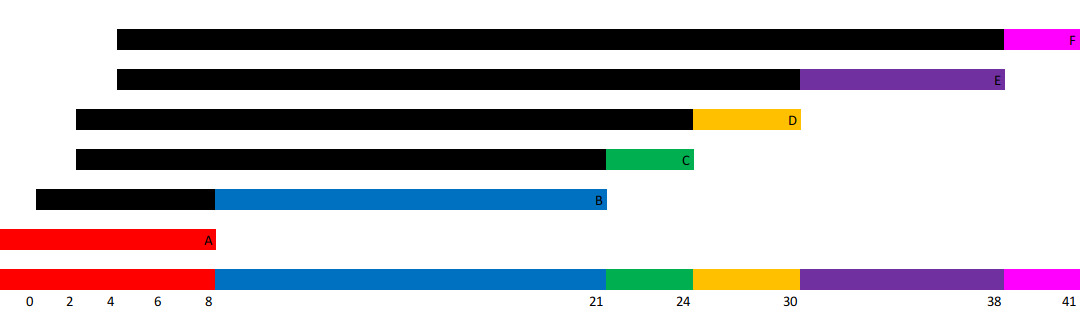
\includegraphics[scale=0.48]{FIFO.jpeg}

faltan los otros dos 

\end{document}